% 动量(高中)
% 动量|冲量|动量定理|动量守恒定律|碰撞

\pentry{牛顿运动定律\upref{HSPM03}}

\subsection{动量}

物体的质量和速度的乘积叫做\textbf{动量},是体现运动物体作用效果的物理量\footnote{进一步理解可参考 “动量和能量、一维势能曲线\upref{CM1}” 的\autoref{CM1_sub1}.}, 表达式为:
\begin{equation}
\bvec p = m\bvec v
\end{equation}

动量是一个矢量,单位为千克米每秒($\mathrm{kg\cdot m/s}$),方向与速度方向相同.

质量为 $m$ 的物体,在恒定合外力 $\bvec F $ 的作用下做匀变速直线运动,速度由 $\bvec v_1$ 变为 $\bvec v_2$,则其动量变化为:
\begin{equation}\label{HSPM08_eq2}
\Delta \bvec p =\bvec p_2 - \bvec p_1 = m\bvec v_2 - m\bvec v_2 = m\Delta \bvec v
\end{equation}

\subsection{冲量}

力和力的作用时间的乘积叫做力的\textbf{冲量},是体现力在其作用时间上积累效果的物理量,表达式为:
\begin{equation}
\bvec I=\bvec F \Delta t
\end{equation}

冲量的单位为牛秒($\mathrm{N\cdot s}$),与动量的单位相同:$1\mathrm{N\cdot s}=1\mathrm{kg\cdot m/s^2 \cdot s}=1\mathrm{kg\cdot m/s}$.

恒力的冲量,可用上式求解;变力的冲量,其计算可考虑分解为多个恒力作用的阶段、计算力—时间图像上对应图形的面积(力的方向恒定时)、求平均力再代入计算或使用动量定理(\autoref{HSPM08_eq3}  )等方法.

\subsection{动量定理}

物体在一个过程中所受力的冲量等于它在这个过程始末的动量变化量.

对于\autoref{HSPM08_eq2} 所述情况,若速度的变化所用时间为 $\Delta t$,则动量的变化率为:
\begin{equation}\label{HSPM08_eq1}
\frac{\Delta \bvec p}{\Delta t}=\frac{m\Delta v}{\Delta t}=m\bvec a=\bvec F
\end{equation}

可见动量的变化率等于合外力.

由\autoref{HSPM08_eq1} 可得:
\begin{equation}\label{HSPM08_eq3}
\bvec I=\bvec F\Delta t=\Delta \bvec p
\end{equation}

与动能定理类似,上述推导同样适用于物体受变力作用的情况.

\subsection{动量守恒定律}

如果一个系统\footnote{由两个或多个相互作用的物体构成的整体叫做一个\textbf{力学系统}(简称\textbf{系统}).系统中物体间的作用力叫做\textbf{内力},系统以外的物体施加给系统内物体的力叫做\textbf{外力}.}不受外力,或所受合外力为零,那么这个系统的总动量保持不变.

推导:在光滑的水平面上有质量分别为 $m_1$ 和 $m_2$ 的甲、乙两个物体在沿同一直线上同向运动(甲在前,乙在后),速度分别为 $\bvec{v_1}$ 和 $\bvec{v_2}$,且 $v_2>v_1$,经过一定时间后,乙追上甲发生碰撞.碰撞过程中,甲受到乙对它的作用力为 $\bvec {F_1}$,乙受到甲对它的作用力为 $\bvec {F_2}$,相互作用的时间 $\Delta t$ 极短.碰撞后甲和乙的速度分别为 $\bvec{v_1'}$ 和 $\bvec{v_2'}$.

根据牛顿第三定律可知:
\begin{equation}\label{HSPM08_eq4}
\bvec {F_1}=-\bvec{F_2}
\end{equation}

对甲、乙两个物体分别使用动量定理可得:
\begin{equation}\label{HSPM08_eq5}
\bvec{F_1}\Delta t=m_1\bvec{v_1'}-m_1\bvec{v_1}
\end{equation}

\begin{equation}\label{HSPM08_eq6}
\bvec{F_2}\Delta t=m_2\bvec{v_2'}-m_2\bvec{v_2}
\end{equation}

联立\autoref{HSPM08_eq4} 、\autoref{HSPM08_eq5} 和\autoref{HSPM08_eq6} 可得:
\begin{equation}
m_1\bvec{v_1}+ m_2\bvec{v_2}= m_1\bvec{v_1'}+ m_2\bvec{v_2'}
\end{equation}


\subsection{碰撞}

两个或以上有相对速度的物体相遇时,在极短时间内发生强烈相互作用,它们的运动状态发生明显的变化,这个过程叫做\textbf{碰撞}.碰撞问题一般都较为复杂,高中阶段以同一直线上的碰撞问题为主.

在碰撞过程中,作用时间极短,速度突变时发生的位移可以忽略不计.另外,系统的内力极大,外力对于内力而言也可以忽略不计,系统的总动量守恒.

根据碰撞后系统机械能的变化情况,碰撞可分为\textbf{弹性碰撞}(系统机械能守恒)和\textbf{非弹性碰撞}(系统机械能减少).非弹性碰撞中,机械能损失最多的情况叫做\textbf{完全非弹性碰撞}.可以理解为:碰撞时两个物体发生了形变,若能完全恢复原状,则系统没有机械能损失,碰撞前后系统机械能守恒;若碰撞后不能完全恢复原状,则系统中有一部分机械能转化为其他形式的能量,碰撞前后系统机械能不守恒(碰撞后系统机械能减少).

\subsubsection{弹性碰撞}
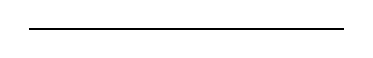
\begin{tikzpicture}
\draw[thick] (0,0)--(4,0);
\end{tikzpicture}

两物体发生弹性碰撞时,系统的总动量守恒,机械能守恒:

\begin{equation}
m_1v_1+m_2v_2=m_1v_1'+m_2v_2'
\end{equation}

\begin{equation}
\frac12m_1v_1^2+\frac12m_2v_2^2=\frac12m_1v_1'^2+\frac12m_2v_2'^2
\end{equation}

解,得

\begin{equation}
v_1'= \frac{2m_2v_2 + (m_1 - m_2)v_1}{m_1+m_2}
\end{equation}
\begin{equation}
v_2'= \frac{2m_1v_1 + (m_2 - m_1)v_2}{m_1+m_2}
\end{equation}

讨论:

1.若$m_1=m_2$,则有$v_1'=v_2$,$v_2'=v_1$即交换速度.

2.若$m_1\gg m_2$,则有$v_1'\approx v_1$,$v_2'\approx v_2+2v_1$

\subsubsection{非弹性碰撞}

两物体发生非弹性碰撞时,系统的总动量守恒,有一部分机械能转化为其他形式的能量,碰撞后系统的机械能减少:

\begin{equation}
m_1v_1+m_2v_2=m_1v_1'+m_2v_2'
\end{equation}

\begin{equation}
\Delta E = E_{k0}-E_{kt}
\end{equation}

$\Delta E$ 为系统的机械能减少量,$E_{k0}$、$ E_{kt}$ 分别为碰撞前、后系统的总动能.

\subsubsection{完全非弹性碰撞}

两物体发生完全非弹性碰撞后,合在一起以共同速度 $\bvec {v'}$ 运动,这种情况下系统的机械能损失最多:

\begin{equation}
m_1v_1+m_2v_2=(m_1+m_2)v'
\end{equation}

\begin{equation}
\Delta E=\frac12m_1v_1^2+\frac12m_2v_2^2-\frac12(m_1+m_2)v'^2
\end{equation}

\addTODO{经典模型}